\documentclass[12pt]{article}
\usepackage{enumitem}
%\usepackage[T1]{fontenc}
\usepackage[auth-sc,affil-sl]{authblk}
\usepackage{amsmath}
\usepackage{graphicx}
\usepackage{color}
\usepackage[toc,page]{appendix}
%\usepackage{enumerate}
\usepackage[round]{natbib}
%\usepackage{url} % not crucial - just used below for the URL 
%\usepackage{amsthm}
\usepackage{amssymb}
\usepackage{graphicx}
\usepackage{epstopdf}
\usepackage{hyperref}
\usepackage{alltt}
\usepackage{listings}
\usepackage{array}
\usepackage[noline, boxed, linesnumbered, procnumbered, titlenumbered]{algorithm2e}
%\usepackage[firstpage]{draftwatermark}
\usepackage[margin=1in]{geometry}  %%jcgs has own margins
\usepackage{lmodern}
\usepackage{caption}
\usepackage{subcaption}

%\pdfminorversion=4
% NOTE: To produce blinded version, replace "0" with "1" below.
\newcommand{\blind}{0}

\newcommand{\secref}[1]{Section~\ref{#1}}
\newcommand{\appdxref}[1]{Appendix~\ref{#1}}
\newcommand{\tblref}[1]{Table~\ref{#1}}
\newcommand{\figref}[1]{Figure~\ref{#1}}
\newcommand{\thmref}[1]{Theorem~\ref{#1}}
\newcommand{\algref}[1]{Algorithm~\ref{#1}}
\newcommand{\funref}[1]{Function~\ref{#1}}
\newcommand{\listingref}[1]{Listing~\ref{#1}}

\newcommand{\eg}{{\em e.g.}}
\newcommand{\ith}{$i^{th}$}
\newcommand{\cut}[1]{}
\newcommand{\todo}[1]{{{\color{red}{[#1]}}}}

\newcommand{\Ex}{\mathop{\mathbb{E}}}
\newcommand{\Imp}{\mathbf{I}}

\newcommand{\spd}{\fontfamily{cmr}\textsc{\small StratPD}}
\newcommand{\cspd}{\fontfamily{cmr}\textsc{\small CatStratPD}}
\newcommand{\xnc}{$x_{\overline{c}}$}
\newcommand{\xnC}{$x_{\overline{C}}$}

\setlist[enumerate]{itemsep=-1mm}

% DON'T change margins - should be 1 inch all around.
\cut{
\addtolength{\oddsidemargin}{-.5in}%
\addtolength{\evensidemargin}{-.5in}%
\addtolength{\textwidth}{1in}%
\addtolength{\textheight}{1.3in}%
\addtolength{\topmargin}{-.8in}%
}

\begin{document}

\def\spacingset#1{\renewcommand{\baselinestretch}%
{#1}\small\normalsize} \spacingset{1}


%%%%%%%%%%%%%%%%%%%%%%%%%%%%%%%%%%%%%%%%%%%%%%%%%%%%%%%%%%%%%%%%%%%%%%%%%%%%%%

\if0\blind
{
  \title{\bf Feature Importance without Models\\
  {\small or feature importance directly from the data? model-free?}}

  \author{Terence Parr and James D. Wilson\\
      University of San Francisco\\
}
  \maketitle
} \fi

\if1\blind
{
  \bigskip
  \bigskip
  \bigskip
  \begin{center}
    {\LARGE\bf Title}
\end{center}
  \medskip
} \fi

\bigskip
\begin{abstract}
dsf
\end{abstract}

\noindent%
{\it Keywords:} feature importance, partial dependence, model interpretability, linear models
%\vfill

%\newpage
%\spacingset{1.5} % DON'T change the spacing!
\section{Introduction}
\label{sec:intro}

Among data analysis techniques, feature importance is one of the most  useful. Data science practitioners use feature importance to gain business insights (e.g., identifying product characteristics valued by customers) and to select features for predictive models (dropping the least predictive features to simplify and potentially increase the generality of the model). While some approaches work directly on the data, such as principle component analysis (PCA), almost all feature importance algorithms analyze data through interrogation of a specific  fitted model, or even interrogating subsidiary models to analyze such fitted models (LIME, SHAP, permutation, drop column).

Relying on a fitted model raises a number of issues. First, practitioners must choose an appropriate model that captures the relationship between features and target. Inaccurate models do not yield useful feature importance results, but there is no definition of ``accurate enough.'' More importantly, it is possible to get very different feature importances running the same algorithm on the same data, just by choosing a different model. This fact is troubling and calls into question the validity of importances derived from fitted models using any technique.  

Consider the feature importance graphs in \figref{fig:diff-models} derived from four different models on the same, well-known Boston toy data set, as computed by SHAP \cite{shap} that has recently emerged as the front runner in feature importance. The linear model (a) struggles to capture the relationship between features and target ($R^2$=0.74), so those importances should not be trusted.  In contrast, the random forest (b), boosted trees (c), and support vector machine (d) models capture the relationship in the training records (all 506) with high fidelity, but SHAP derives meaningfully different feature importances from each model.  This is particularly true given the high variance of the importances computed from the random forest. \todo{explain that} It is unclear which results, if any, are correct. If humans could examine the data directly to find the true feature importances, we would not need feature importance algorithms. (we'll intro fitness measure in \secref{foo}.)

\begin{figure}[htbp]
\begin{center}
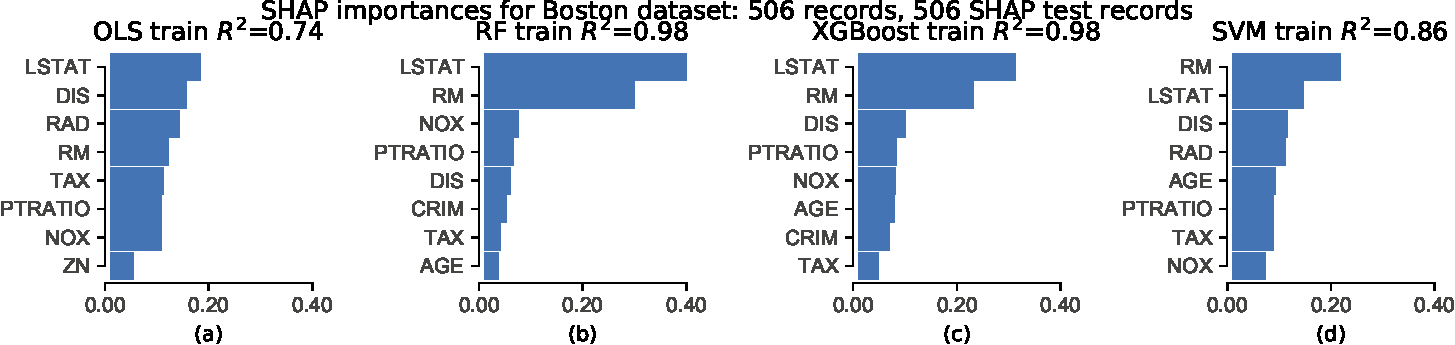
\includegraphics[scale=0.6]{images/diff-models.pdf}
\caption{Top 8 of 13 features. {\tt\footnotesize RandomForestRegressor(n\_estimators=30)}, {\tt\footnotesize XGBRegressor(max\_depth=5, eta=0.01, n\_estimators=50)}, {\tt\footnotesize SVR(gamma=0.001, C=100)} High var for RF. nshap=n test records. Rough timing for explaining 506 test records is (a) less than 1 second, (b) 10s, (c) 3s, and (d) 50s.}
\label{fig:diff-models}
\end{center}
\end{figure}

The differences clearly arise because the feature importances are distorted by the lens of the models. Current techniques peer through the model (and possibly through an extra, explanatory model) to the underlying data, but true feature importances are relationships that exist in the data, with or without a model.  For example, to gain business insights about customers, a predictive model is unnecessary and a data analysis technique that revealed importances directly would be sufficient. \todo{maybe say PCA does this although limited to linear features and assumes most spread = most important?} Besides, predictive features do not always coincide with important features; e.g., some models are unable to capture nonlinear relationships and, therefore, always find them non-predictive.  \todo{last bit redundant?}
 
In our experience, it is best to get importances using multiple techniques and to view the combined results as a clue rather than the gospel truth.  The unfortunate reality is that practitioners routinely make business decisions and  perform feature selection using the results provided by machine learning libraries without questioning their validity.  For example, \cite{rfpimp} demonstrated that the widely-used {\em gini-drop} technique, specific to random forests, gives inappropriate weight to features with many unique values, even pure noise features. (The gini-drop of a feature is the average drop in gini impurity for decision nodes splitting on that feature.)

Despite many years of research attention, there is still no widely-held definition of feature importance. While there are multiple precisely-defined algorithms with known strengths and weaknesses, all interrogate fitted models for predictions. The primary contributions of this paper are (1) a simple definition of feature importance that is purely a function of training data and (2) an implementation that yields plausible and effective results, as measured by the {\em top-p} fitness metric defined in \secref{foo}.

~\\
\noindent \todo{Likely a good spot for a paper walk-through}

\section{A definition of feature importance}\label{sec:def}

For true function $y = f(\bf x)$ and ${\bf x} = [x_1, \ldots, x_p]$ and ${\bf X} = [x^{(1)}, \ldots, x^{(n)}]$ (skipping bolding the vectors there).  Training data is pair ($\bf X, y$).

The partial dependence of $y$ on  $x_i$ is the isolated contribution of $x_i$ to $y$. At some $x_j=z$ value, the partial dependence is the cumulative sum of $\frac{\partial y}{\partial x_j}$ from $min(x_j)$ up to $z$:

\[
\text{\it PD}_j(z) = \int_{min(x_j)}^z \frac{\partial y}{\partial x_j} dx_j
\]

Software currently relies on something like:

\[
\Ex[\text{\it PD}_j] = \frac{1}{N} \sum_{i=1}^{N} \text{\it PD}_j(x_j^{(i)})
\]

\[
\Imp_j = \Ex[|\text{\it PD}_j|]
\]

or normalized 0..1 as:

\[
\Imp_j = \frac{\Ex[|\text{\it PD}_j|]}{\Ex[y]}
\]

\noindent where

\[
\Ex[y] = \sum_{j=1}^p \Ex[\text{\it PD}_j]%\big |_{min(x_j)}^{max(x_j)}
\]

or, with less accurate PDP (to keep 0..1) since

\[
\Imp_j = \frac{\Ex[|\text{\it PD}_j|]}{\sum_{k=1}^p \Ex[|\text{\it PD}_k|]}
\]

Here is where we show that SHAP gets $y = x_1^2 + x_2 + 100$ wrong.
 
\section{foo}

 what is the definition: loosely as which are most predictive

The variance of the importances derived from the random forest is high, SHAP has specialized ``explainers'' for linear and tree-based models for performance reasons, but relies on the general method to explain support vector machines. , but the results are subject to the variance of the internal model parameters.  Ideally, feature importances would not change from run to run on the same data set using the same technique.

\bibliographystyle{apalike}

\bibliography{pdimp}
\end{document}